%
%	Section 2: The client API
%

\section{The \TitularMbrace{} Client API}
\label{sec:client}

The \mbrace{} framework comes with a rich client API that provides access to the 
following functionalities:
\begin{enumerate}
\item The cloud workflow programming model and primitives, as presented in section
\ref{sec:workflows}.
\item An interface for managing and interacting with the \mbrace{} runtime, 
that can be roughly divided in the following categories:
	\begin{itemize}
		\item Runtime administration functionality, that includes cluster management
		operations such as initialization, halting, health monitoring and
		real-time elastic node management.
		\item Cloud process management functionality, that includes submission of
		computations, process monitoring, debugging and storage access.
	\end{itemize}

%\item The \mbrace{} shell, which enables interactive declaration of cloud computations
%	and runtime administration.
\item A collection of command line tools for server-side deployments.
\item A rich open source library that includes a range of combinators that
implement common parallelism patterns like MapReduce or Choice and a multitude of 
sample implementations of real-world algorithms.
\end{enumerate}
%
The client API can be consumed either programmatically from native \dotnet{} code
or interactively using the \mbox{\mbrace{}} shell. The \mbrace{} interactive shell is
an adaptation of the interpreter that comes with the open source \fsharp{} compiler
distribution. It permits direct, on-the-fly declaration and submission of cloud 
computations to the data center. Capitalizing on the IDE integration capabilities 
offered by \fsharp{} interactive, \mbrace{} offers a cloud programming experience%
\footnote{For a demo, see \samehref{http://www.youtube.com/watch?v=fmTagG6MNPQ}.}
that fully integrates with development environments such as Visual Studio,
Xamarin Studio or the Tsunami IDE%
\footnote{\mbrace{} with Tsunami, \samehref{http://www.youtube.com/watch?v=fjssBxpNqrU}}.

\begin{figure}[ht]
\label{shellfig}
\centering
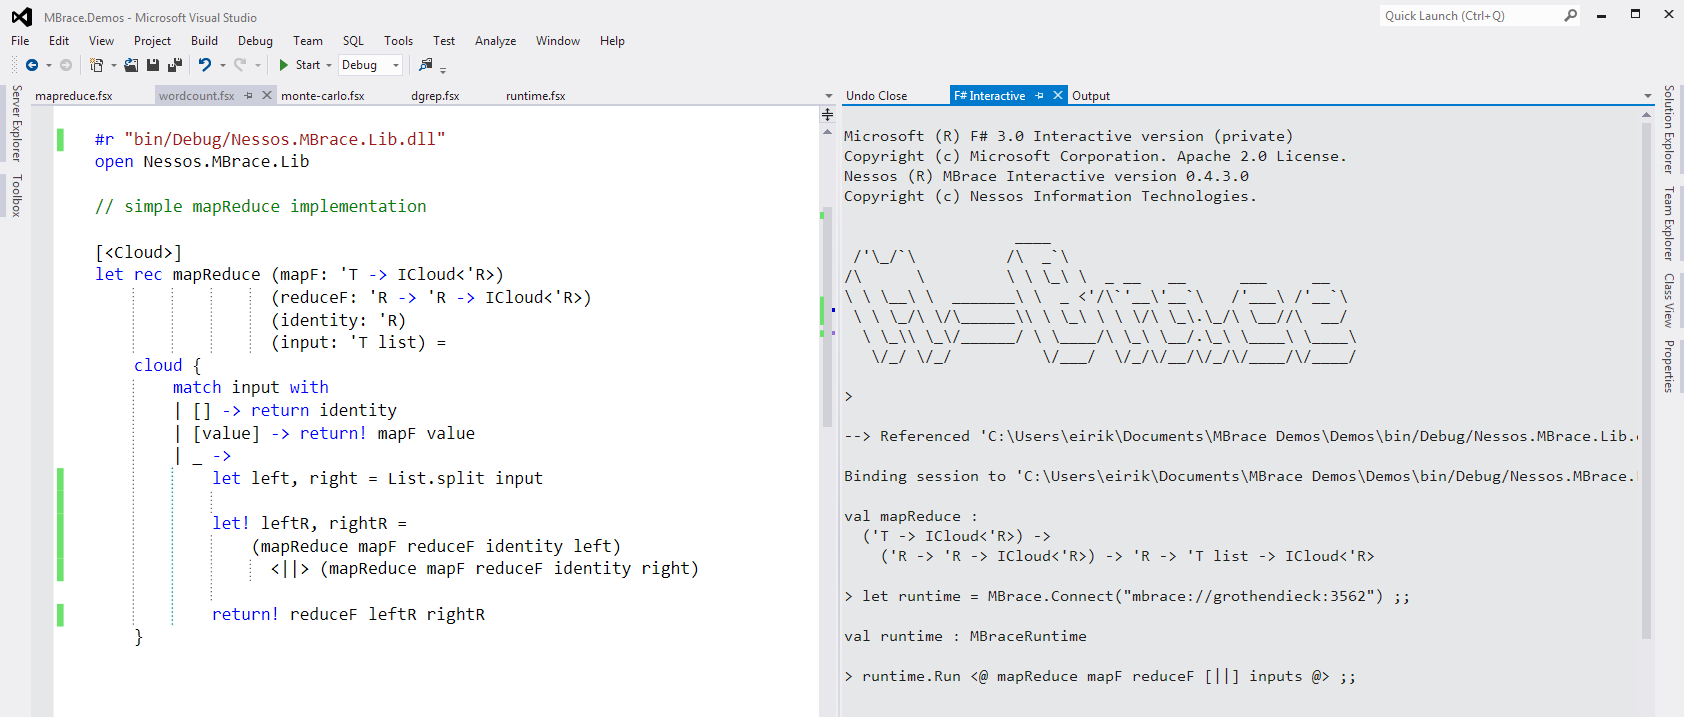
\includegraphics[width=\textwidth]{shell.png}
\caption{The \Mbrace{} Shell integrated with Visual Studio.}
\end{figure}

\subsection{The Cloud Workflow API}
\label{sec:client:workflows}

Cloud workflows can be declared using the syntax and primitives as described in section \ref{sec:workflows}.
In this segment we offer some additional information on cloud workflows that relate to the client API.

\subsubsection*{Quotations \& the Cloud Attribute}

The primary function of the \mbrace{} client stack is traversing cloud workflows for dependencies,
then gathering the corresponding \dotnet{} library files before everything is uploaded to the cloud
for execution. This dependency traversal is achieved with the help of \fsharp{} code quotations.

As demonstrated earlier, cloud computations in \mbrace{} need to be initialized like so:
\begin{lstlisting}
let proc = runtime.CreateProcess <@ cloud { return 1 + 1 } @>
\end{lstlisting}
where \texttt{runtime} denotes a client object to a running \mbrace{} cluster.
A peculiar feature of this syntax is that cloud blocks are delimited by \texttt{<@} and 
\texttt{@>} symbols. These are part of the \fsharp{} language feature known as \emph{code quotations}%
\footnote{\fsharp{} Code Quotations, \samehref{http://msdn.microsoft.com/en-us/library/dd233212.aspx}}.
Any \fsharp{} expression enclosed in these symbols will yield a
typed \emph{syntax tree} of the given expression, also known as its \emph{quotation}.
The quotation expression \texttt{<@ 1 + 1 @>} has type \texttt{Expr<int>}, meaning that it is a syntax 
tree which, if evaluated, will yield a result of type \texttt{int}.

The \texttt{CreateProcess} method in \mbrace{} has type signature
\centertt{Expr<Cloud<\uq{}T>> -> Process<\uq{}T>}
which means that all executed cloud blocks need to be quoted.
This does not mean that all cloud computations have to be enclosed in quotation symbols:
only the top-level expression need be so:
\begin{lstlisting}
[<Cloud>]
let test () = cloud { return 1 }

runtime.Run <@ test () @>
\end{lstlisting}

Despite this, all nested calls to cloud workflows need to be affixed with a \texttt{[<Cloud>]}
attribute. Failing to do so will result in a runtime error being raised.
The \texttt{CloudAttribute} is just an abbreviation of the \texttt{ReflectedDefinitionAttribute}%
\footnote{See, \samehref{http://msdn.microsoft.com/en-us/library/ee353643.aspx}}
provided by \fsharp{}. Adding this to a declaration makes the \fsharp{} compiler generate a 
reflected quotation to the tagged code.

It should be noted that the \texttt{Cloud} attribute is not mandatory for \fsharp{} declarations that
are not cloud workflows. For example, the following code is perfectly valid:
\begin{lstlisting}
let f x = x + 1

[<Cloud>]
let g () = cloud { return f 41 }
\end{lstlisting}

Code quotations are an excellent resource for metadata and as such, they are mandatory
in cloud workflows. Among others, they are utilized for extracting library dependencies,
variable names, nesting patterns, etc.

\subsubsection*{The \TitularMbrace{} Shell}

The \mbrace{} shell is an adapted version of the open source \fsharp{} interactive.
It allows for ad hoc declaration of cloud workflows directly from the REPL, that
can then be submitted to the cloud for execution. This is made possible through
a custom mechanism that compiles accumulated REPL interactions into static assemblies,
which can then be sent to remote machines for execution.
\begin{verbatim}
   > [<Cloud>] let f x = cloud { return 2 * x } ;;

   val f : unit -> Cloud<int>

   > runtime.Run <@ f 21 @> ;;
   compiling interactions to assembly... 
   uploading assemblies to runtime... 
   val it : int = 42
   >
\end{verbatim}
The \mbrace{} shell is also capable of including custom types to computations.
\begin{verbatim}
   > type Container = Content of int ;;

   type Container = | Content of int

   > match runtime.Run <@ cloud { return Content 42 } @> with
   | Content 42 -> printfn "success"
   | _ -> printfn "failure" ;;
   compiling interactions to assembly... 
   uploading assemblies to runtime... 
   success
   val it : unit = ()
\end{verbatim}


\subsubsection*{Value Declarations \& Side Effects}

We now describe a technical issue that is related to the distributed nature of cloud computation.
Consider a library that includes the following code:
\begin{lstlisting}
let data = System.IO.File.ReadAllBytes "/Users/eirik/Desktop/1.dat"

[<Cloud>]
let getSize () = cloud { return data.Length }

let run () = runtime.Run <@ getSize () @>
\end{lstlisting}
One might hold the expectation that the \texttt{data} will be read at the client side,
with the cloud workflow segment of the computation taking place at the runtime.
This is not the case however: in fact, \texttt{data} will be read \emph{in every}
node of the runtime separately. This can lead to unanticipated errors, in this case
having to do with the fact that \texttt{1.dat} does only exist in the client computer.

The problem occurs because \texttt{data} is a library artifact, not something
that relates to client-side execution explicitly. In the \fsharp{} compiler in particular,
let-bound values are initialized using underlying static constructors, which are triggered
whenever the parent library gets used, be it the client or the runtime.
Since \mbrace{} distributes depended libraries to all worker nodes, type initialization 
side-effects are going to be triggered everywhere.

Value initialization issues can be typically resolved by demoting such values from top-level
declarations:
\begin{lstlisting}
[<Cloud>]
let getSize (data : byte []) = cloud { return data.Length }

let run () = 
	let data = System.IO.File.ReadAllBytes "/Users/eirik/Desktop/1.dat" in
	runtime.Run <@ getSize data  @>
\end{lstlisting}

An important exception to the above behaviour is the \mbrace{} shell. The shell has the 
important property that both compilation and execution take place in the same process. 
Moreover, patterns like the one described above are very common in repl environments.
This has allowed us overcome the above problem for certain data types using a technique
that involves code erasure of value initializers in the assemblies compiled by the shell.

While this works well for most grounded types, erasure in higher-order types such as lambdas,
object expressions and workflows is not possible, often resulting in a warning message being 
output by the shell:
\begin{verbatim}
    > let f = () ; fun x -> x + 1
	
   val f : int -> int

   > runtime.Run <@ cloud { return f 41 } @>
   Warning: Cloud block encloses value 'f'. Consider converting to a function.
   val it : int = 42
\end{verbatim}
In this case, the warning occurs since the \fsharp{} compiler represents \texttt f with
a \dotnet{} property, rather than a method. The simplest workaround would be to convert 
the value into a thunk, or adopting an argument passing style as in the example
given previously.

\subsubsection*{Non-Serializable Objects}

\noindent Consider the following snippet:
\begin{lstlisting}
cloud {
	let http = new System.Net.WebClient()
	let download url = cloud { return http.DownloadString url }
	return! 
		Cloud.Parallel <| 
			Array.map download 
				[| "http://www.m-brace.net" ; "http://www.nessos.gr" |]
}
\end{lstlisting}
This workflow is clearly wrong, since it demands the distribution of an evidently
nondistributable local resource, an instance of \texttt{WebClient}.
In fact, attempting to submit this workflow to a runtime for execution will result in
an error, since the client will detect that it uses instances of non-serializable 
types.

Cloud workflows do not support environments with non-serializable objects,
and for good reason. So how does one integrate code that utilizes types such
as file streams, web sockets, etc?
%
The answer is to encapsulate locally scoped objects in an execution context
that enforces local semantics. This can be done using native \fsharp{} code:
\begin{lstlisting}
let download (url : string) =
	use http = new System.Net.WebClient()
	http.DownloadString url

cloud {
	return! Cloud.Parallel <|
		Array.map (fun u -> cloud { return download u })
			[| "http://www.m-brace.net" ; "http://www.nessos.gr" |]
}
\end{lstlisting}
or by embedding \texttt{async} workflows:
\begin{lstlisting}
let downloadAsync (url : string) = async {
	use http = new System.Net.WebClient()
	return! http.DownloadStringAsync url
}

cloud {
	return! Cloud.Parallel <|
		Array.map (Cloud.OfAsync << downloadAsync)
			[| "http://www.m-brace.net" ; "http://www.nessos.gr" |]
} 
\end{lstlisting}

The above coding style reflects the operation philosophy of \mbrace:
cloud workflows ought to be restricted to the orchestration of distribution patterns, 
whereas computation taking place within the context of a single worker 
had preferably be elaborated in native \dotnet{} or async workflows.

\subsubsection*{Local Execution}

In absence of a runtime, cloud workflows can be executed locally using the method
%
\centertt{MBrace.RunLocal : Cloud<\uq{}T> -> \uq{}T}
%
This will run the workflow in a local interpreter with execution semantics that resemble
but do not coincide with those of Async: while distribution does occur through thread 
concurrency, it differs in certain subtleties that are introduced artificially so that 
the execution model of the \mbrace{} runtime is more closely emulated.
For more information, please refer to the \href{peculiarities}{``Semantic Peculiarities''}
segment of section \ref{sec:workflows}.

\subsection{Managing \TitularMbrace{} Runtimes}

The \mbrace{} runtime is a cluster of connected computers capable of orchestrating the execution
of cloud workflows. Every computer participating in an \mbrace{} runtime is known as an \mbrace{}
\emph{node}. In this section we offer an overview of how the \mbrace{} client stack can be
used to initialize, manage and monitor remote \mbrace{} runtimes.

\subsubsection*{The \texttt{MBraceNode} Type}

An \mbrace{} \emph{node} represents any physical machine that runs the \emph{\mbrace{}} daemon, 
the server-side component of the framework. Every \mbrace{} daemon accepts connections from a predetermined 
\texttt{tcp} port on the host. \Mbrace{} nodes are identifiable by the uri format
\centertt{mbrace://hostname:port/}
The \mbrace{} client can connect to a remote node by calling
\begin{lstlisting}
let node = Node("mbrace://hostname:2675")
\end{lstlisting}
or equivalently,
\begin{lstlisting}
let node = Node("hostname", 2675)
\end{lstlisting}
This will initialize an object of type \texttt{MBraceNode}. This object acts as a handle
to the remote node. It can be used to perform a variety of operations like
\begin{lstlisting}
node.Ping() // ping the node, returning the number of milliseconds taken
\end{lstlisting}
or
\begin{lstlisting}
node.IsActive : bool
\end{lstlisting}
which is a property indicating whether the node is part of an existing \mbrace{} cluster.

Every \mbrace{} daemon writes to a log of its own. \Mbrace{} node logs can accessed remotely
from the client either in the form of a dump
\begin{lstlisting}
node.ShowLogs()
\end{lstlisting}
or in a structured format that can be used to perform local queries:
\begin{lstlisting}
node.GetLogs() 
|> Seq.filter (fun log -> log.DateTime > DateTime.Now - TimeSpan.FromDays 1.0)
\end{lstlisting}

\subsubsection*{The \texttt{MBraceRuntime} Type}

An \mbrace{} runtime can be \emph{booted} once access to a collection of at least two nodes,
all running within the same subnet, has been established. This can be done like so:
\begin{lstlisting}
let nodes = [ Node("host1", 2675) ; Node("host2", 2675) ; Node("host3", 2675) ]

let runtime = MBraceRuntime.Boot nodes
\end{lstlisting}
This will initialize an \mbrace{} cluster and will return a client handle of type
\texttt{MbraceRuntime}. 
%
To connect to an already booted \mbrace{} runtime, one needs simply write
\begin{lstlisting}
let runtime = MBraceRuntime.Connect("mbrace://host:port/")
\end{lstlisting}
wherein the supplied uri can point to any of the constituent worker nodes.

The client stack provides a facility for instantaneously spawning local runtimes:
\begin{lstlisting}
let runtime = MBraceRuntime.InitLocal(totalNodes = 4, background = true)
\end{lstlisting}
This will initiate a runtime of four local nodes that execute in the background.
The feature is particularly useful for quick deployments of distributed code under development.

The \texttt{MBraceRuntime} object serves as the entry point for any kind of client interactions 
with the cluster. For instance, the property
\begin{lstlisting}
runtime.Nodes : Node list
\end{lstlisting}
returns the list of all nodes that constitute the cluster.
In the \mbrace{} shell, calling
\begin{lstlisting}
runtime.ShowRuntimeInfo()
\end{lstlisting}
prints a detailed description of the cluster to the terminal.
\begin{verbatim}
   {m}brace runtime information (active)                                               

   Host           Port  Role        Location          Connection String            
   ----           ----  ----        --------          -----------------            
   grothendieck  38857  Master      Local (Pid 3008)  mbrace://grothendieck:38857/ 
   grothendieck  38873  Alt Master  Local (Pid 3616)  mbrace://grothendieck:38873/ 
   grothendieck  38865  Alt Master  Local (Pid 4952)  mbrace://grothendieck:38865/ 
\end{verbatim}
The state of the runtime can be reset or stopped at any point by calling the following methods:
\begin{lstlisting}
runtime.Shutdown() // stops the runtime
runtime.Reboot() // resets the state of the runtime
runtime.Kill() // violently kills all node processes in the runtime
\end{lstlisting}

\subsection{Managing Cloud Processes}

A \emph{cloud process} is a currently executing or completed cloud computation in the context
of a specific \mbrace{} runtime. In any given runtime, cloud processes can be initialized,
monitored for progress, or cancelled; completed cloud processes can be queried for their results
and symbolic stack traces can be fetched for failed executions.

Cloud processes form a fundamental organizational unit for the \mbrace{} runtime:
conceptually, if one is to think of \mbrace{} as an operating system for the cloud,
then cloud processes form its units of distributed execution;
every cloud process spawns its own set of scheduler and workers;
the \mbrace{} runtime enforces a regime of \emph{process isolation},
which means that each cloud process will run in a distinct instance of the CLR in the context
of each worker node.

Given a \emph{runtime} object, a cloud process can be initialized like so:
\begin{lstlisting}
let proc = runtime.CreateProcess <@ cloud { return 1 + 1 } @>
\end{lstlisting}
This will submit the workflow to the runtime for execution and return with a process handle of
type \texttt{Process<int>}. Various useful properties can be used to query the status of the
cloud computation at any time. For instance,
\begin{lstlisting}
proc.Result // Pending, Value, user Exception or system Fault
proc.ProcessId // the cloud process id
proc.InitTime // returns a System.DateTime on execution start
proc.ExecutionTime // returns a System.TimeSpan on execution time
proc.GetUserLogs() // get user logs for cloud process
\end{lstlisting}
If running in the \mbrace{} shell, typing the command
\begin{verbatim}
   > proc.ShowProcessInfo() ;;
\end{verbatim}
will print information like the following
\begin{verbatim}
 Name       Process Id  Status   #Workers  #Tasks  Start Time         Result Type       
 ----       ----------  ------   --------  ------  ----------         -----------       
 mapReduce        6674  Running         2       2  30/7/2013 4:08:21  (string * int) [] 
\end{verbatim}
Similar to \texttt{CreateProcess} is the \texttt{Run} method:
\begin{lstlisting}
let result : int = runtime.Run <@ cloud { return 1 + 1 } @>
\end{lstlisting}
This is a blocking version of \texttt{CreateProcess} that is equivalent to the statement below:
\begin{lstlisting}
let proc = runtime.CreateProcess <@ cloud { return 1 + 1 } @> in
proc.AwaitResult()
\end{lstlisting}
%
The \texttt{AwaitResult} method also comes in an asynchronous flavour
\begin{lstlisting}
let task : Task<int> = proc.AwaitResultAsync() |> Async.StartAsTask
\end{lstlisting}
%
A list of all executing cloud processes in a given runtime can be obtained as follows:
\begin{lstlisting}
let procs : Process list = runtime.GetAllProcesses()
\end{lstlisting}
This will return a list of \emph{untyped} cloud process handles. The untyped process handle
is a supertype of the typed version and can be downcast like so:
\begin{lstlisting}
let proc' = proc.Cast<int> ()
\end{lstlisting}
If running in the \mbrace{} Shell, process information can be printed to the buffer like so:
\begin{verbatim}
   > runtime.ShowProcessInfo() ;;
\end{verbatim}
Given a cloud process id, one can receive the corresponding handle object like so:
\begin{lstlisting}
let proc : Process = runtime.GetProcess 1131
let proc' : Process<string> = runtime.GetProcess<string> 119
\end{lstlisting}
Finally, an executing cloud process can be cancelled with the following method
\begin{lstlisting}
proc.Kill()
\end{lstlisting}

\subsection{\TitularMbrace{} Client Settings}

Certain aspects of the \mbrace{} client can be configured by the user.
This is done through the \texttt{MBraceSettings} fa\c{c}ade that contains an
assortment of property getters and setters:
\begin{itemize}
\item The \texttt{MBraceSettings.ClientId} property returns a Guid that is
associated with the current client instance. This is used internally by \mbrace{} to
track client sessions and efficiently manage user assemblies.
\item The \texttt{MBraceSettings.AssemblyCachePath} gets or sets the local system 
path in which the client caches user generated assemblies.
\item The boolean \texttt{MBraceSettings.ClientSideExpressionCheck} enables or 
disables cloud workflow static checks on the client side. This feature is reserved
for system debugging purposes.
\item The \texttt{MBraceSettings.LocalCachePath} gets or sets the local system path
in which items like cloud refs or cloud files are cached with the client.
\item The \texttt{MBraceSettings.MBracedExecutablePath} gets or sets the path to the
local \texttt{mbraced} executable. This is used by the client to spawn local instances
of \mbrace{} nodes.
\item The \texttt{MBraceSettings.StoreProvider} gets or sets the global store provider
in which the client connects to. Please refer to the runtime section of this document
for further information. NB: this particular interface is subject to change.
\end{itemize}
